
\mode*

\begin{frame}<presentation>[label=FrameHerramientas]{Herramientas Alternativas}

\begin{columns} 

\column{0.5\textwidth}
\begin{center}

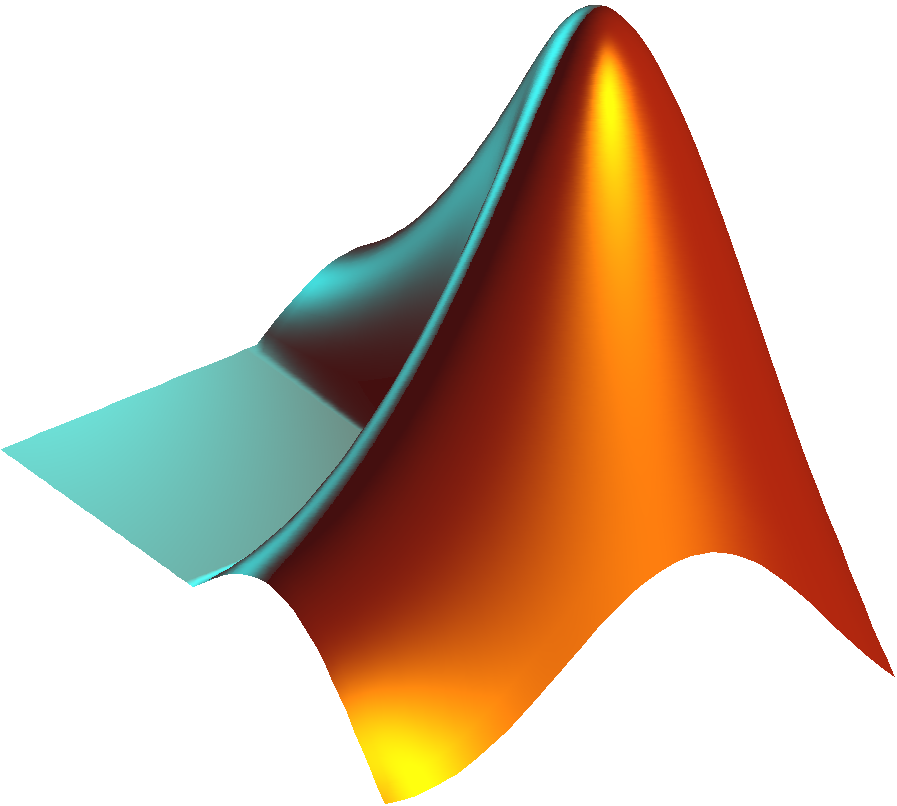
\includegraphics[height=1cm]{./media/Matlab_Logo.png}
\LARGE Matlab \par
\vspace{1cm} 

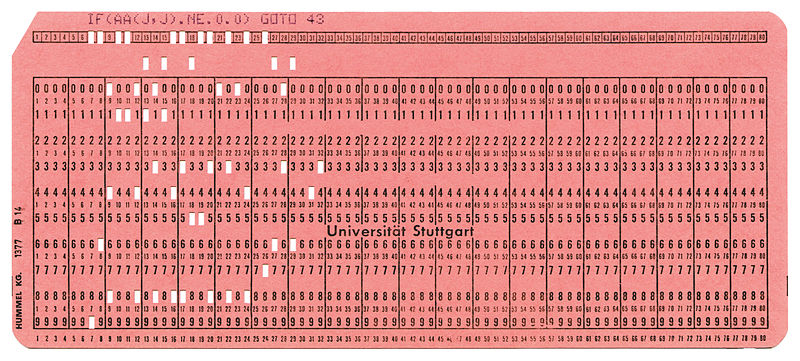
\includegraphics[height=1cm]{./media/punch.jpg}
\LARGE Fortran \par
\vspace{1cm} 


\includegraphics[height=1cm]{./media/scipyshiny_small.png}
\LARGE Python / SciPy \par
\end{center}

\column{0.5\textwidth}

\begin{center}


\includegraphics[height=1cm]{./media/logo_octave.png}
\LARGE Octave \par
\vspace{1cm} 

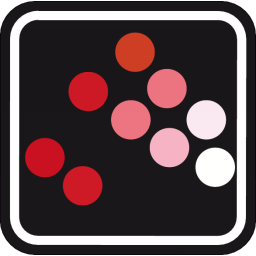
\includegraphics[height=1cm]{./media/scilab.png}
\LARGE SciLab \par
\vspace{1cm} 

\onslide<2>{
  
\includegraphics[height=2cm]{./media/fray.jpeg}
}
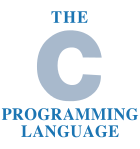
\includegraphics[height=2cm]{./media/The_C_Programming_Language_logo.png}

\end{center}

\end{columns}

\end{frame}

\mode<all>
